%----------------------------------------------------------------------------------------
%	PACKAGES AND THEMES
%----------------------------------------------------------------------------------------

\documentclass{beamer}
\mode<presentation> {
	\usetheme{Warsaw}
	\setbeamercolor{page_num_color}{fg=white,bg=blue}

	\defbeamertemplate*{footline}{shadow theme}{%
		\leavevmode%
		\hbox{\begin{beamercolorbox}[wd=.5\paperwidth,ht=2.5ex,dp=1.125ex,leftskip=.3cm plus1fil,rightskip=.3cm]{author in head/foot}%
		    \usebeamerfont{author in head/foot}\hfill\insertshortauthor
		\end{beamercolorbox}%
		\begin{beamercolorbox}[wd=.4\paperwidth,ht=2.5ex,dp=1.125ex,leftskip=.3cm,rightskip=.3cm plus1fil]{title in head/foot}%
		    \usebeamerfont{title in head/foot}\insertshorttitle\hfill%
		\end{beamercolorbox}%
		\begin{beamercolorbox}[wd=.1\paperwidth,ht=2.5ex,dp=1.125ex,leftskip=.3cm,rightskip=.3cm plus1fil]{author in head/foot}%
		\hfill\insertframenumber\,/\,\inserttotalframenumber
		\end{beamercolorbox}}%
		\vskip0pt%
	}
}

\usepackage{amsmath}
\usepackage{amssymb}
\usepackage{graphicx} % Allows including images
\usepackage{booktabs} % Allows the use of \toprule, \midrule and \bottomrule in tables
\usepackage[english]{babel}
\usepackage{graphicx}
\usepackage{listings, lstautogobble}
\usepackage{color}
\usepackage{caption}
\usepackage{verbatim}


%----------------------------------------------------------------------------------------
%	LSTSETTING
%----------------------------------------------------------------------------------------
\lstset{language=C,
    keywordstyle=\color{blue}, 
    morekeywords={then},
    numberstyle=\footnotesize,
    basicstyle=\ttfamily\footnotesize,
    numbers=left,
    stepnumber=1,
    frame=single,
    breaklines=true,
    tabsize=4,
    escapeinside={(*}{*)},
    autogobble=true
}

%----------------------------------------------------------------------------------------
%   TITLE PAGE 
%----------------------------------------------------------------------------------------

\title[Bounding Volume Hierarchies of k-DOPs]
{Efficient Collision Detection Using Bounding Volume Hierarchies of k-DOPs} % The short title appears at the bottom of every slide, the full title is only on the title page
\author[James T. Klosowski]
{   James T. Klosowski
} % Your name
\institute[] % Your institution as it will appear on the bottom of every slide, may be shorthand to save space
{
	1998 IEEE Transactions on Visualization and Computer Graphics \\ % Your institution for the title page
 	\bigskip Presenter: Yi-Ning Chang
}
\date{March 29, 2017} % Date, can be changed to a custom date


\begin{document}

%----------------------------------------------------------------------------------------
%	TITLE PAGE SETTING
%----------------------------------------------------------------------------------------
\begin{frame}[noframenumbering]
    \titlepage % Print the title page as the first slide
\end{frame}

\AtBeginSection[]
  {
  	 \setbeamertemplate{footline}{} 
     \begin{frame}<beamer>[noframenumbering]
     \tableofcontents[currentsection, hideallsubsections]
     \end{frame}
     \setbeamertemplate{footline}{%
		\leavevmode%
		\hbox{\begin{beamercolorbox}[wd=.5\paperwidth,ht=2.5ex,dp=1.125ex,leftskip=.3cm plus1fil,rightskip=.3cm]{author in head/foot}%
		    \usebeamerfont{author in head/foot}\hfill\insertshortauthor
		\end{beamercolorbox}%
		\begin{beamercolorbox}[wd=.4\paperwidth,ht=2.5ex,dp=1.125ex,leftskip=.3cm,rightskip=.3cm plus1fil]{title in head/foot}%
		    \usebeamerfont{title in head/foot}\insertshorttitle\hfill%
		\end{beamercolorbox}%
		\begin{beamercolorbox}[wd=.1\paperwidth,ht=2.5ex,dp=1.125ex,leftskip=.3cm,rightskip=.3cm plus1fil]{author in head/foot}%
		\hfill\insertframenumber\,/\,\inserttotalframenumber
		\end{beamercolorbox}}%
		\vskip0pt%
	}
  }


%------------------------------------------------
% Outline
%------------------------------------------------
\begin{frame}
\frametitle{Outline} % Table of contents slide, comment this block out to remove it
\tableofcontents[hideallsubsections] % Throughout your presentation, if you choose to use \section{} and \subsection{} commands, these will automatically be printed on this slide as an overview of your presentation
\end{frame}


%------------------------------------------------
% Introduction
%------------------------------------------------
\section{Introduction}
    \begin{frame}
    \frametitle{Introduction}
	\begin{itemize}
		\item Collision detection is of paramount importance for many applications in computer graphics and visualization.
		\item In this paper, author develop and analyze a method, based on bounding-volumn hierarchies, for efficient collision detection for objects moving within highly complex environments.
		\item Previous work
			\begin{itemize}
			\item Octrees, k-d trees, BSP trees, and so on.
			\item \it{RAPID} (Robust and Accurate Polygon Interference Detection) system based on \it{OBBTrees}.
			\end{itemize}
	\end{itemize}
    \end{frame}

%------------------------------------------------
% BV-Tree
%------------------------------------------------
\section{BV-Tree}

% BV-Tree
\subsection{BV-Tree}
	\begin{frame}
	\frametitle{BV-Tree}
		\begin{itemize}
			\item $BVT(S)$: a BV-tree specifies a bounding volumn hierarchy on $S$.
			\item Set $S$: a set of $n$ geometry triangles in 3D that specify the boundary of polygonal models.
			\item Each node $v$ of $BVT(S)$ corresponds to a subset, $S_{v} \subseteq S$.
			\item $b(S_{v})$: a \it{bounding volume}, associated with node $v$ of $BST(S)$, is an approximation to the set $S_{v}$ using a smallest instance of specified class of shapes.
		\end{itemize}
	\end{frame}

	\begin{frame}
	\frametitle{BV-tree}
		\begin{figure}[h!]
			\centering
			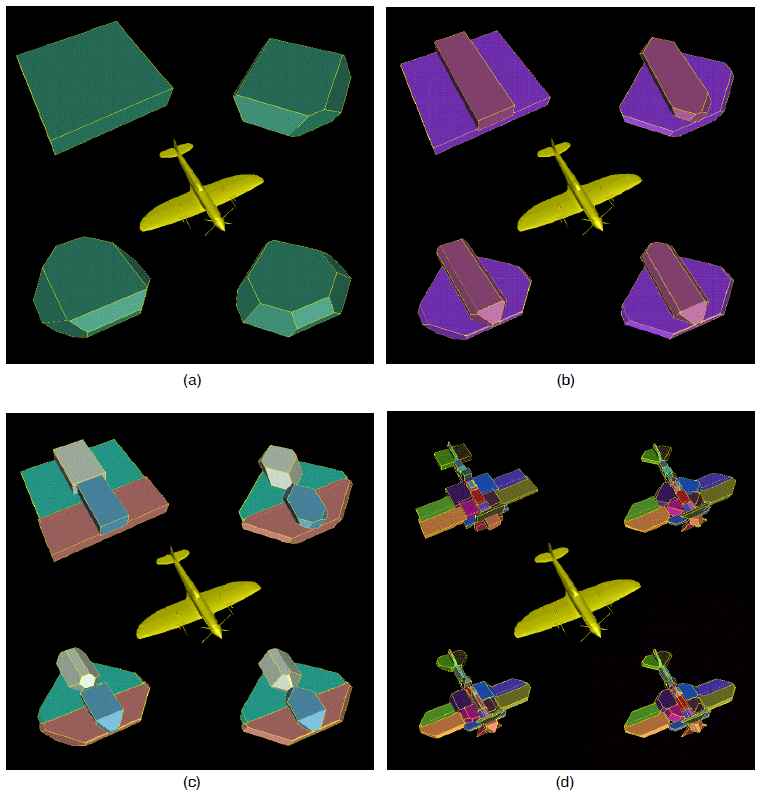
\includegraphics[width=0.6\textwidth]{./figure/BVTrees.PNG}
		\end{figure}
	\end{frame}

% Design Criteria
\subsection{Design Criteria}
	\begin{frame}
	\frametitle{Design Criteria}
		$$T=N_{v} \times C_{v}+N_{p} \times C_{p}+N_{u} \times C_{u}$$
		\begin{itemize}
			\item $T$: total cost function for collision detection.
			\item $N_{v}$: number of pairs of bounding volumes tested for overlap.
			\item $C_{v}$: cost of testing a pair of bounding volumes for overlap.
			\item $N_{p}$: number of pairs of primitives tested for contact.
			\item $C_{p}$: cost of testing a pair of primitives for contact.
			\item $N_{u}$: number of nodes of the flying hierarchy must be updated.
			\item $C_{u}$: cost of updating such node.
		\end{itemize}
	\end{frame}

% k-DOPs
\subsection{k-DOP}
	\begin{frame}
	\frametitle{k-DOP}
		\begin{itemize}
			\item k-dop: \it{k-discrete orientation polytope} is a convex polytope whose facets are determined by $k$ \it{fixed} orientations.
			\item \it{6-dop}(AABB), \it{14-dop}, \it{18-dop}, \it{26-dop}
		\end{itemize}
		\begin{center}
			\begin{tabular}{l || c | c | c}
					& Sphere & AABB & OBB \\
				\hline
				$N_{i}$ & big & median & small\\ 
				$C_{v}$ & $O(1)$ & $O(k)$ & $O(\log^{2}n)$\\
				$C_{u}$ & $O(1)$ & $O(k^{2})$ & $O(1)$\\
			\end{tabular}
		\end{center}
	\end{frame}
	
	\begin{frame}
		\begin{figure}[h!]
			\centering
			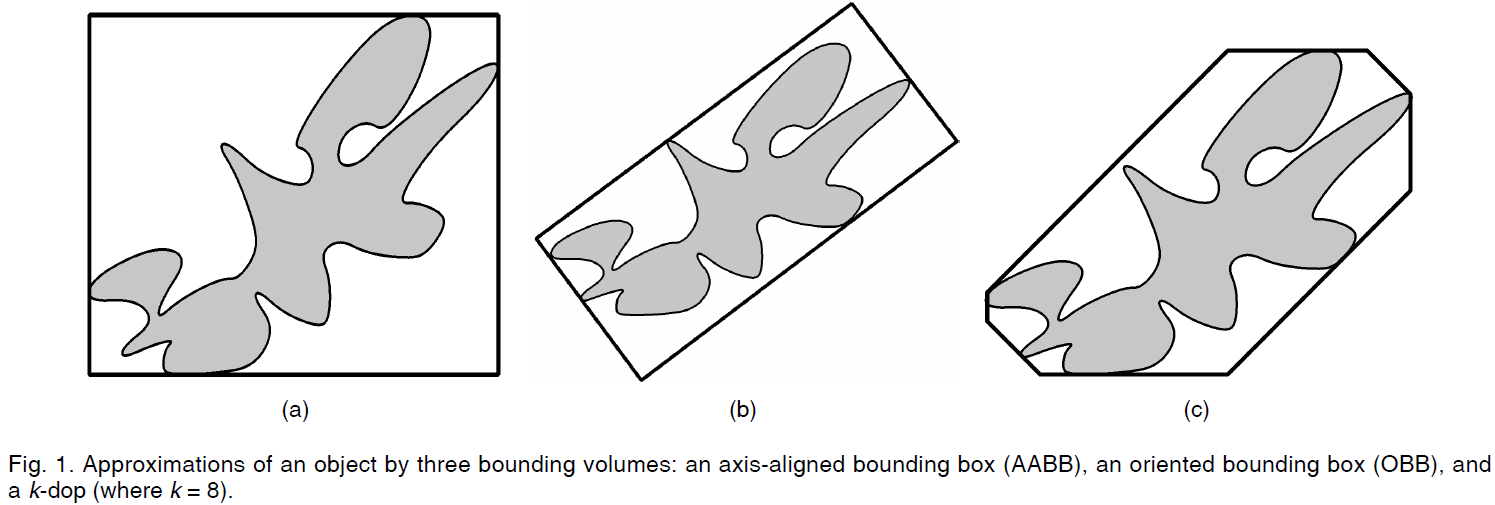
\includegraphics[width=1.0\textwidth]{./figure/kDOPs.PNG}
		\end{figure}
	\end{frame}

% Splitting Rule
\subsection{Splitting Rule}
	\begin{frame}
	\frametitle{Splitting Rule}
		\begin{itemize}
			\item Choice of Axis
			\begin{itemize}
				\item \it{Min Sum}: $O(k|S_{v}|)+O(k\log k)$
				\item \it{Min Max}: $O(k|S_{v}|)+O(k\log k)$
				\item \it{Splatter}: $O(|S_{v}|)$
				\item \it{Longest Side}: $O(1)$
			\end{itemize}
			\item Choice of Split Point
			\begin{itemize}
				\item \it{median}: more balanced.
				\item \it{mean}: less total volume while not harming the balance of the tree severely.
			\end{itemize}
		\end{itemize}
	\end{frame}

%------------------------------------------------
% Collision Detection Using BV-Tree
%------------------------------------------------
\section{Collision Detection}

% Collision Detection Using BV-tree
\subsection{Collision Detection Using BV-Trees}
	\begin{frame}
	\frametitle{Collision Detection Using BV-Trees}
		\begin{itemize}
			\item The method of \it{updating} the k-dops.
			\item The \it{algorithm} for comparing two BV-trees to determine if there is a collision.
			\item The \it{depth} of the hierarchy.
			\item The \it{order} in testing two k-dops for interection.
		\end{itemize}
	\end{frame}

% Update
\subsection{Update}
	\begin{frame}
	\frametitle{Updating the BV-Trees}
	\begin{itemize}
		\item \it{Hill climbing algorithm}
			\begin{itemize}
				\item Store the boundary representation of convex hull of $S_{v}$.
				\item $O(k^{2})$
			\end{itemize}
		\item \it{Approximation method}
			\begin{itemize}
				\item store the boundary vertices of the k-dop $b(S_{v})$.
				\item $O(k\log k)$
			\end{itemize}
	\end{itemize}	
	\begin{figure}
		\centering
		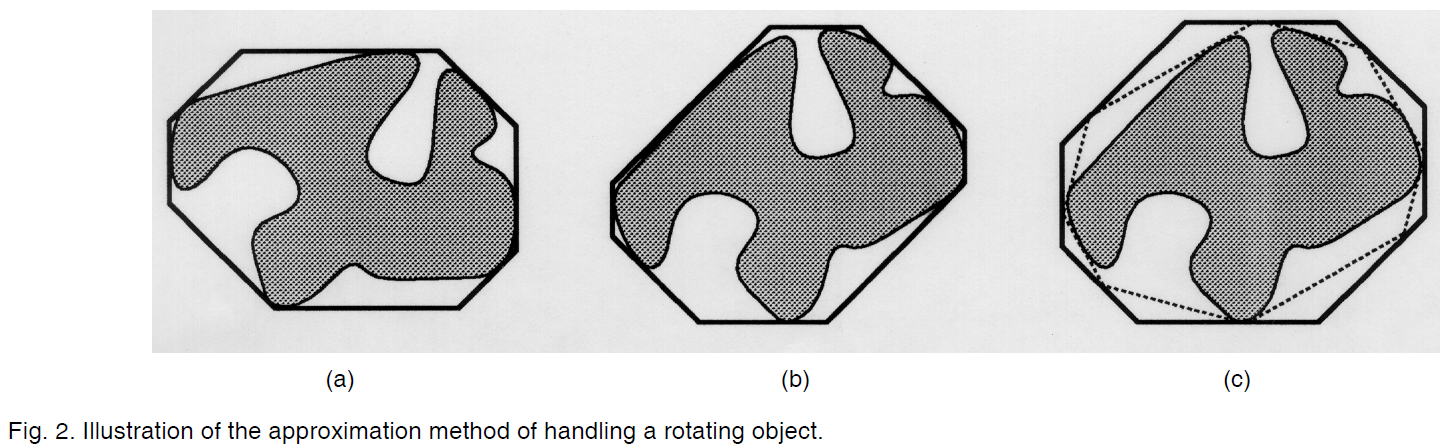
\includegraphics[width=1.0\textwidth]{./figure/update.PNG}
	\end{figure}
	\end{frame}

% CD Algorithm
\subsection{Collision Detection Algorithm}
	\begin{frame}
	\frametitle{Tree Traversal Algorithm}
	\begin{figure}[h!]
		\centering
		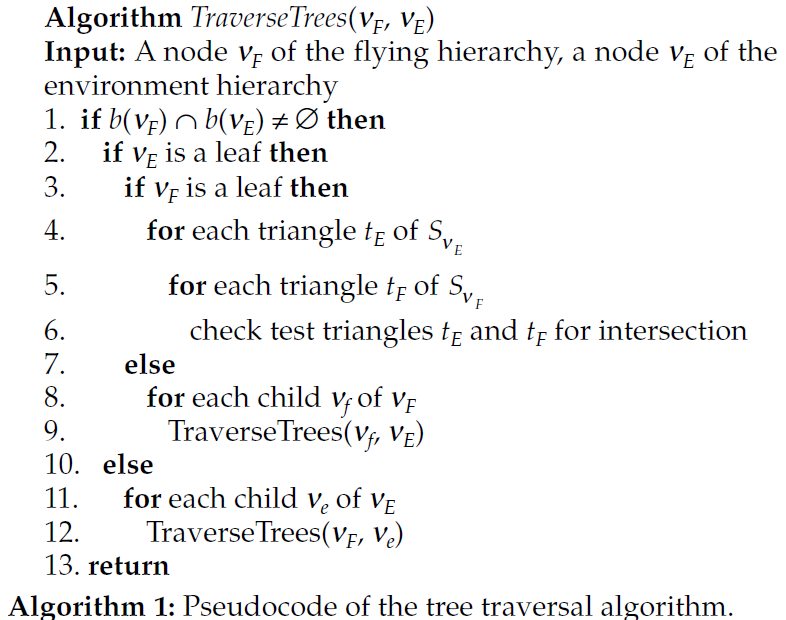
\includegraphics[width=0.7\textwidth]{./figure/algorithm.PNG}
	\end{figure}
	\end{frame}

% Depth of the Hierarchy
\subsection{Depth of the Hierarchy}
	\begin{frame}
	\frametitle{Depth of the Flying Hierarchy}
	\end{frame}

% Overlap and Intersection Tests
\subsection{Overlap and Intersection Test}
	\begin{frame}
	\frametitle{Overlap and Intersection Test}
	\end{frame}

%------------------------------------------------
% Experiment
%------------------------------------------------
\section{Experiment}

% Experiment
\subsection{Experiment}
	\begin{frame}
	\frametitle{Experiment for different k}
	\begin{figure}[h!]
		\centering
		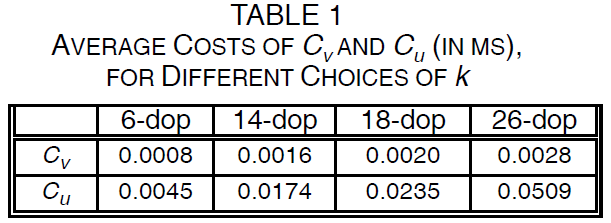
\includegraphics[width=0.5\textwidth]{./figure/TABLE1.PNG}
		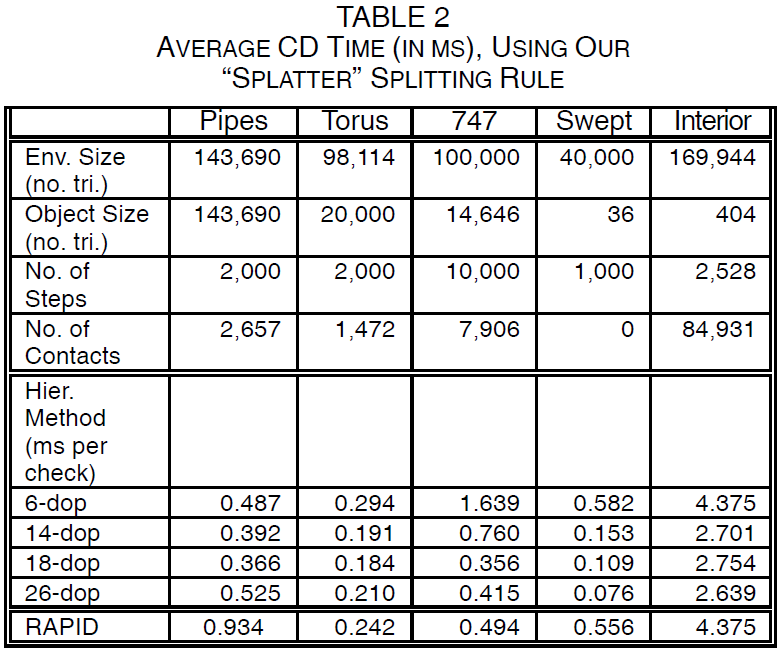
\includegraphics[width=0.5\textwidth]{./figure/TABLE2.PNG}
	\end{figure}
	\end{frame}

	\begin{frame}
	\frametitle{Experiment for preprocessing time}
	\begin{figure}[h!]
		\centering
		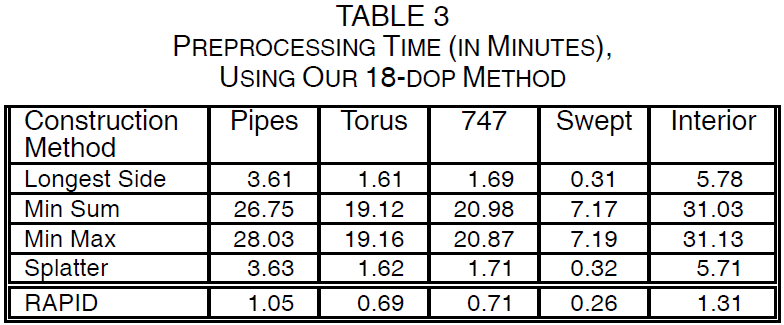
\includegraphics[width=0.7\textwidth]{./figure/TABLE3.PNG}
	\end{figure}
	\end{frame}

	\begin{frame}
	\frametitle{Experiment for dividing method}
	\begin{figure}[h!]
		\centering
		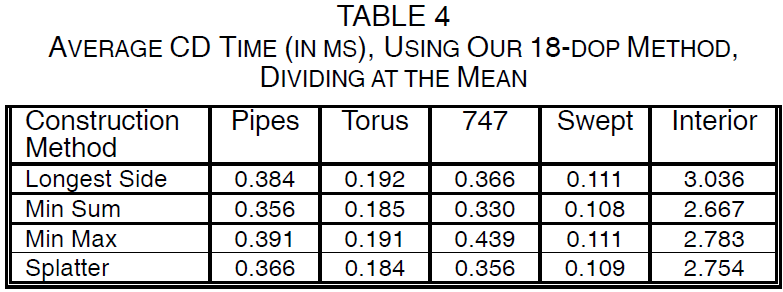
\includegraphics[width=0.7\textwidth]{./figure/TABLE4.PNG}
	\end{figure}
	\begin{figure}[h!]
		\centering
		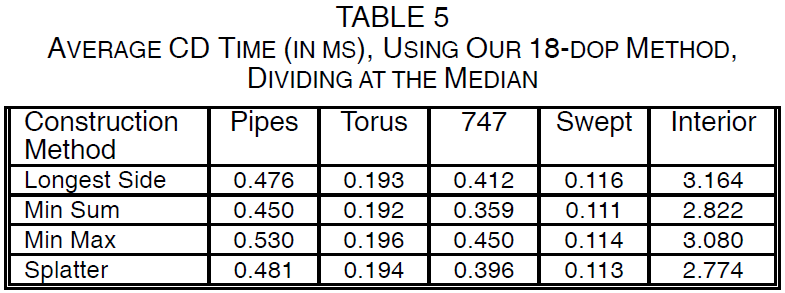
\includegraphics[width=0.7\textwidth]{./figure/TABLE5.PNG}
	\end{figure}
	\end{frame}

%------------------------------------------------
% Conclusion
%------------------------------------------------
\section{Conclusion}

\begin{frame}
\frametitle{Conclusion}
\begin{itemize}
	\item Proposed a method for efficient collision detection among polygonal models, based on a bounding volumes hierarchy (BV-tree) whose bounding volumes are k-dops.
	\item Future work
		\begin{itemize}
		\item Multiple flying objects.
		\item Server and client system.
		\end{itemize}
\end{itemize}
\end{frame}

\end{document} 
